\section{Umsetzung des Proof of Concept}
\label{sec:umsetzung}

Technisch werden das 360°-Cockpit sowie das Governance-Cockpit mittels einer Python Anwendung mit FastAPI implementiert. Die Nutzung des Python Setups begründet sich damit, dass die CLIs von Anbietern wie Azure und AWS auf Python basieren. Des Weiteren ermöglicht FastAPI mit vergleichbar geringem Aufwand einen RESTful Service zu erstellen. Um die Trennung der beiden Cockpit Komponenten zu betonen, passieren gegenseitige Aufrufe jeweils via HTTP Interface. Zur Persistierung verwenden die Komponenten Project Collection, Evidence Collection, Governance Decision Store und Governance Intent Repository eine MongoDB Document Database. Die Wahl einer Document Database begründet sich mit der Abbildung der Traceability-Beziehung als JSON-Objekte, was eine Handhabung aus implementatorischer Sicht vereinfacht. Für den Landing Zone Plattform Configuration Service wird ein statisches IaC Setup mit Terraform verwendet. Die modellierten Traceability-Beziehungen werden hierbei als statischer Inhalt geteilt. Über das Setup hinaus werden weitere Cloud-Ressourcen erzeugt welche in einem funktionalen Setup bereits als gegeben angenommen werden:

\begin{itemize}
    \item Techinsche Benutzer / Service Accounts für die automatisierte wie manuelle Provisionerung von Cloud-Ressourcen
    \item Verrechnungsstruktur als Vorraussetzung zur Erzeugung von Subscriptions/Accounts
    \item Initiale Subcriptions/Accounts für Komponentn welche über verschiedenen Landing-Zones hinweg verwendet werden (bspw. Analytics Workspace)
\end{itemize}

Die Traceability-Beziehungen werden basierend auf dem Basismodell in \fullref{sec:trace-arch-variant2} modelliert und im Rahmen der Umsetzung adaptiert. Für den Scope im \ac{poc} wird 

\begin{figure}[H]
    \centering
    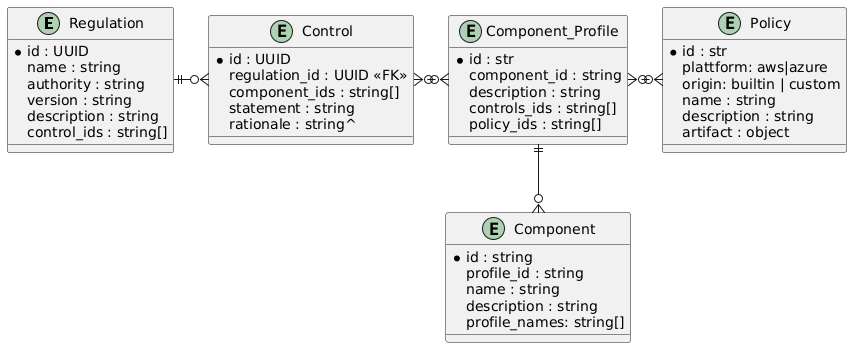
\includegraphics[width=\textwidth]{graphics/poc_data_model.png}
    \caption{Datenmodell für Traceability-Beziehung im \ac{poc}}
    \label{fig:data-model-poc}
\end{figure}


% @startuml
% entity "Regulation" as regulation {
%   *id : UUID
%   name : string
%   authority : string
%   version : string
%   description : string
%   control_ids : string[]
% }

% entity "Control" as control {
%   *id : UUID
%   regulation_id : UUID <<FK>>
%   component_ids : string[]
%   statement : string
%   rationale : string^
% }

% entity "Policy" as policy {
%   *id : str
%   plattform: aws|azure
%   origin: builtin | custom
%   name : string
%   description : string
%   artifact : object
% }

% entity "Component_Profile" as component_profile {
%   *id : str
%   component_id : string
%   description : string
%   controls_ids : string[]
%   policy_ids : string[]
% }

% entity "Component" as component {
%   *id : string
%   profile_id : string 
%   name : string
%   description : string 
%   profile_names: string[]
% }


% regulation ||-right-o{ control
% component_profile ||--o{ component
% control }o-right-o{ component_profile
% policy }o-left-o{ component_profile
% @enduml